\documentclass{standalone}
\usepackage{amsmath}
\usepackage{pgfplots}
\usetikzlibrary{arrows}

\begin{document}

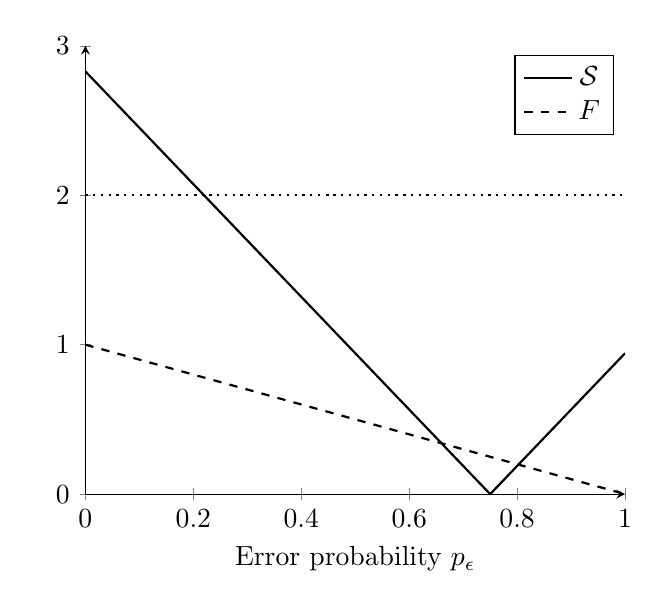
\begin{tikzpicture}
\begin{axis}[
    axis lines = left,
    ymin = 0,
    ymax = 3,
    xlabel = Error probability \(p_{\epsilon}\),
    ylabel = {\(\)},
]
%Below the red parabola is defined
\addplot [
    domain=0:1, 
    samples=500, 
    color=black,
    thick,
]
{4/2^(1/2) * abs((1 - 4 * x /3))};
\addlegendentry{\(\mathcal{S}\)}
%Here the blue parabola is defined
\addplot [
    domain=0:1, 
    samples=50, 
    color=black,
    thick,
    dashed,
    ]
    {1-x};
\addlegendentry{\(F\)}

\addplot [
    domain=0:1,
    samples=50,
    color=black,
    thick,
    dotted
  ]
  {2};

\end{axis}
  
\end{tikzpicture}

\end{document}